\documentclass{standalone}
\usepackage{ tikz }
\usepackage{ xparse }
\usepackage{../../macros}

\begin{document}
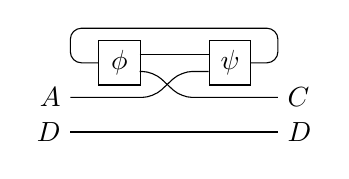
\begin{tikzpicture}[yscale=-1,x=1em,y=1.25em]

    \node [anchor=east] at (0,1.5) {$A$};
    \node [anchor=east] at (0,2.5) {$D$};

    \draw [rounded corners] (0,1.5) -- (3,1.5) -- (4,0.75) -- (5,0.75);
    \draw [] (0,2.5) -- (7.5,2.5);

    \node[draw, minimum height = 1.6em, minimum width = 1.5em, anchor = west] at (1,0.5){$\phi$};

    \draw [] (2.5,0.25) -- (5,0.25);
    \draw [rounded corners] (2.5,0.75) -- (3,0.75) -- (4,1.5) -- (7.5,1.5);
    \draw [rounded corners] (6.5,0.5) -- (7.5,0.5) -- (7.5,-0.5) -- (0,-0.5) -- (0,0.5) -- (1,0.5);
    
    \node[draw, minimum height = 1.6em, minimum width = 1.5em, anchor = west] at (5,0.5){$\psi$};

    \node [anchor=west] at (7.5,1.5) {$C$};
    \node [anchor=west] at (7.5,2.5) {$D$};
\end{tikzpicture}
\end{document}